\documentclass[12pt,a4paper]{article}
\usepackage[a4paper,margin=1in]{geometry}
\setlength{\headheight}{15pt}
\usepackage{graphicx}
\usepackage{booktabs}
\usepackage{amsmath,amssymb}
\usepackage{float}
\usepackage{hyperref}
\usepackage{xcolor}
\usepackage{listings}
\usepackage{enumitem}
\usepackage{fancyhdr}
\usepackage{longtable}

\hypersetup{colorlinks=true,linkcolor=blue,urlcolor=blue}

\pagestyle{fancy}
\fancyhf{}
\lhead{ICS1512}
\rhead{Machine Learning Algorithms Laboratory}
\cfoot{\thepage}

\lstset{
language=Python,
basicstyle=\ttfamily\footnotesize,
numbers=left,
numberstyle=\tiny\color{gray},
frame=single,
breaklines=true,
showstringspaces=false,
keywordstyle=\color{blue},
commentstyle=\color{gray},
stringstyle=\color{red}
}

\begin{document}

\begin{tabular}{|p{4cm}|p{11cm}|}
\hline
Experiment No. & 8\\ \hline
Experiment Title & Clustering Analysis using K-Means, DBSCAN, and Hierarchical Clustering\\ \hline
GitHub Repository & \href{https://github.com/rishirithesh/ML_Lab}{Click Here} \\ \hline
Jupyter Notebook & \href{https://github.com/rishirithesh/ML_Lab/blob/main/MLEXP8.ipynb}{Click Here to View MLEXP8.ipynb} \\ \hline
Student Name & Rishi Rithesh\\ \hline
Register Number & 3122247001049\\ \hline
Faculty & Dr. Poreddy Ajay Kumar Reddy \\ \hline
Submission Date & 21/09/2026\\ \hline
\end{tabular}

\vspace{0.4cm}

\section{Objective}
To explore, implement, and rigorously benchmark the primary unsupervised clustering paradigms—\textbf{Partition-based} (K-Means), \textbf{Density-based} (DBSCAN), and \textbf{Hierarchical} (Agglomerative Clustering)—on the high-dimensional Human Activity Recognition (HAR) dataset. Specific objectives include:
\begin{enumerate}[label=\alph*)]
    \item Performing Exploratory Data Analysis, feature scaling, and non-linear dimensionality reduction (PCA and t-SNE) on 561-dimensional sensor measurements.
    \item Implementing K-Means clustering and determining the optimal cluster count $k$ using the \textbf{Elbow Method} (Within-Cluster Sum of Squares, WCSS) and \textbf{Silhouette Analysis}.
    \item Implementing DBSCAN and tuning density parameters ($\epsilon$ and $minPts$) via sorted $k$-nearest neighbor distance graphs and noise ratio monitoring.
    \item Evaluating Hierarchical Agglomerative Clustering across \textbf{Ward, Complete, Average, and Single} linkage criteria and visualizing cluster topologies using truncated dendrograms.
    \item Benchmarking clustering quality across intrinsic metrics (\textit{Silhouette Score, Davies-Bouldin Index, Calinski-Harabasz Score}) and extrinsic ground-truth alignment metrics (\textit{Adjusted Rand Index [ARI], Normalized Mutual Information [NMI]}).
\end{enumerate}

\section{Problem Statement}
\textbf{Problem:} To partition unlabeled smartphone accelerometer and gyroscope sensor telemetry into coherent clusters corresponding to human physical activities (e.g., dynamic movements vs. static postures) without supervised label guidance, comparing how centroid, density, and connectivity algorithms perform in high-dimensional continuous feature spaces.

\textbf{Input:} The UCI Human Activity Recognition (HAR) dataset consisting of 7,352 training instances characterized by 561 temporal and spectral domain features extracted from triaxial body acceleration and angular velocity signals.

\textbf{Output:} Standardized feature representations, optimal parameter search tables for K-Means and DBSCAN, hierarchical dendrograms, 2D PCA and t-SNE cluster scatter visualizations, multi-metric performance evaluation tables, comparative radar/bar visualizations, and the complete executable Python implementation.

\section{Dataset Description}
\begin{longtable}{|p{6cm}|p{8cm}|}
\hline
Dataset Name & UCI Human Activity Recognition (HAR) Dataset\\ \hline
Dataset Source & UCI Machine Learning Repository\\ \hline
Number of Samples ($N$) & 7,352 training observations\\ \hline
Number of Features ($p$) & 561 continuous variables (time \& frequency domain)\\ \hline
Sensor Modalities & Triaxial Accelerometer and Triaxial Gyroscope (50 Hz)\\ \hline
True Activity Classes ($K=6$) & LAYING, SITTING, STANDING, WALKING, WALKING\_DOWNSTAIRS, WALKING\_UPSTAIRS\\ \hline
Missing Values & None (verified \& median-checked)\\ \hline
Preprocessing Applied & Z-score Standardization (\texttt{StandardScaler})\\ \hline
Subspace Reductions & PCA (2D for plotting, 50D for DBSCAN), t-SNE (2D)\\ \hline
\end{longtable}

\section{Exploratory Data Analysis and Subspace Projections}
\begin{itemize}
    \item Univariate feature distributions and density estimation of sensor signals
    \item Ground truth activity visualization in 2D linear PCA projection
    \item Non-linear manifold visualization using t-Distributed Stochastic Neighbor Embedding (t-SNE)
\end{itemize}

\subsection*{Figure: Feature Distributions}
\begin{figure}[H]
\centering
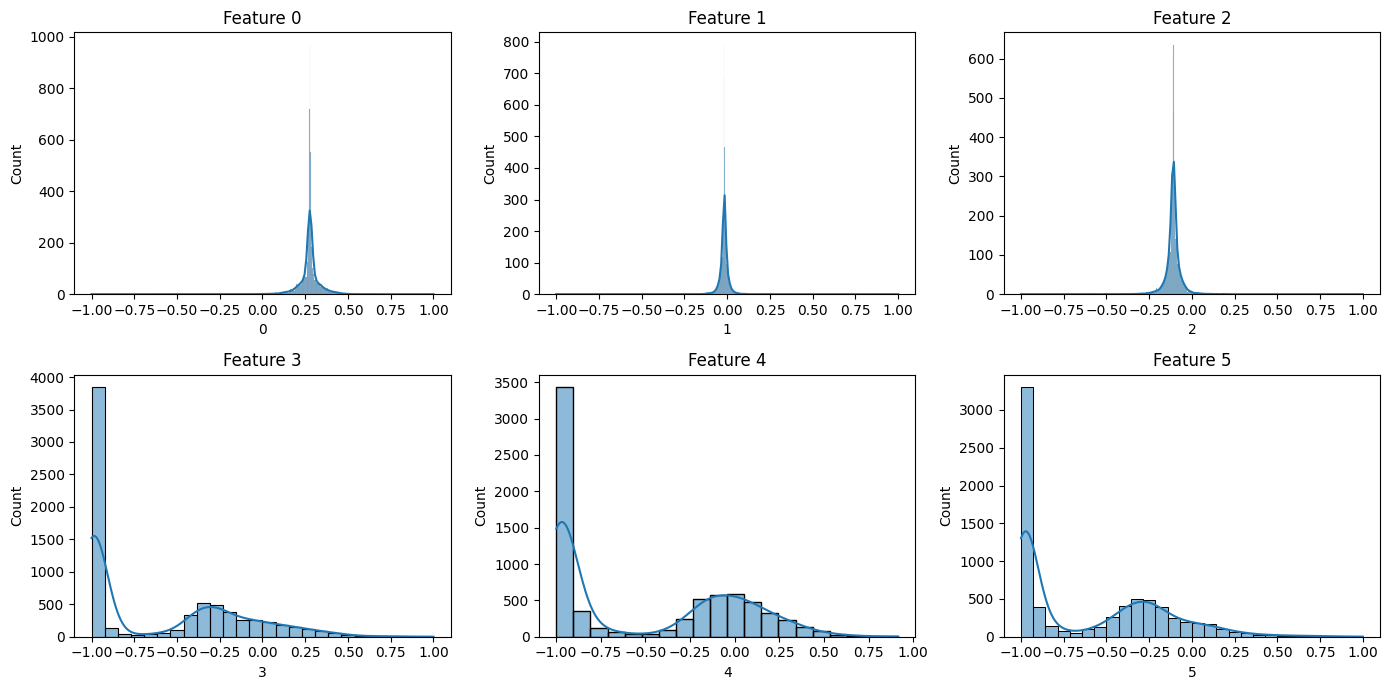
\includegraphics[width=0.85\linewidth]{har_feature_distributions.png}
\caption{Probability Density and Histograms for the First Six Time-Domain Telemetry Features}
\end{figure}

\textbf{Inference:}
The initial continuous features exhibit multimodal and bounded distributions (ranging within $[-1, 1]$), reflecting gravitational and oscillatory motion components. Standardizing these inputs ensures equal contribution across distance calculations in clustering algorithms.

\subsection*{Figure: Ground Truth Activities in PCA and t-SNE Projections}
\begin{figure}[H]
\centering
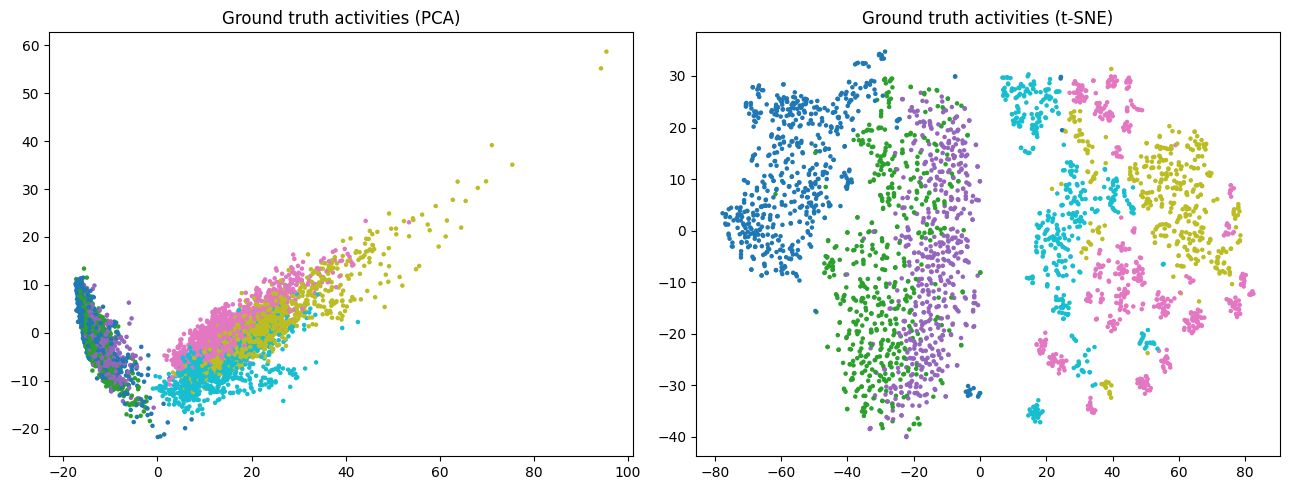
\includegraphics[width=0.9\linewidth]{har_ground_truth_pca_tsne.png}
\caption{Ground Truth Activity Class Projections in 2D PCA (Left) and 2D t-SNE (Right)}
\end{figure}

\textbf{Inference:}
Both PCA and t-SNE reveal a primary macro-separation dividing the 6 activities into two distinct super-clusters: \textbf{Dynamic Activities} (Walking, Walking Upstairs, Walking Downstairs) and \textbf{Static Postures} (Laying, Sitting, Standing). The non-linear t-SNE embedding exhibits tighter local cluster cohesion, illustrating why linear clustering methods predominantly split the data into $k=2$ primary modes.

\section{Data Preprocessing and Mathematical Methodology}
\begin{itemize}
    \item \textbf{Feature Standardization:} Features are normalized to zero mean and unit variance ($\mathbf{z} = (\mathbf{x} - \boldsymbol{\mu}) / \boldsymbol{\sigma}$), which is critical for Euclidean distance-based clustering algorithms.
    \item \textbf{Dimensionality Reduction for Density Estimation:} For DBSCAN, the curse of dimensionality causes distance concentration in 561 dimensions. A 50-component PCA transformation ($\mathbf{X}_{50}$) retaining $>85\%$ variance is used to define density neighborhoods reliably.
    \item \textbf{t-SNE Embedding:} A random subsample of $N=3000$ points is projected onto 2D space with perplexity 30 to visually evaluate non-linear cluster geometry.
\end{itemize}

\section{K-Means Clustering Analysis}
K-Means minimizes the Within-Cluster Sum of Squares (WCSS / Inertia):
\begin{equation}
J = \sum_{j=1}^k \sum_{\mathbf{x}_i \in C_j} \|\mathbf{x}_i - \boldsymbol{\mu}_j\|^2
\end{equation}
K-Means was executed for $k \in \{2, 3, 4, 5, 6, 7, 8\}$ with 10 random initializations ($n\_init=10$).

\begin{table}[H]
\centering
\caption{K-Means Clustering: Number of Clusters vs. WCSS and Silhouette Score}
\label{tab:kmeans_metrics}
\begin{tabular}{|c|c|c|}
\hline
\textbf{Cluster Count ($k$)} & \textbf{Within-Cluster Sum of Squares (WCSS)} & \textbf{Silhouette Score}\\ \hline
\textbf{2} & \textbf{2,336,223.75} & \textbf{0.397}\\ \hline
3 & 2,081,849.63 & 0.327\\ \hline
4 & 1,976,450.56 & 0.163\\ \hline
5 & 1,875,065.69 & 0.132\\ \hline
6 & 1,818,833.96 & 0.110\\ \hline
7 & 1,776,046.02 & 0.104\\ \hline
8 & 1,735,669.99 & 0.083\\ \hline
\end{tabular}
\end{table}

\subsection*{Figure: K-Means Elbow Curve and Silhouette Spectrum}
\begin{figure}[H]
\centering
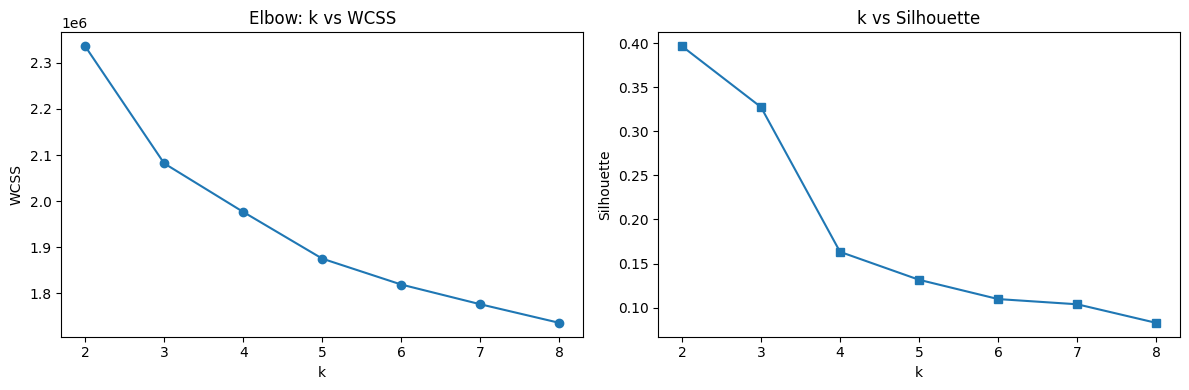
\includegraphics[width=0.85\linewidth]{kmeans_elbow_silhouette.png}
\caption{Elbow Plot of WCSS vs. $k$ (Left) and Silhouette Score vs. $k$ (Right)}
\end{figure}

\textbf{Inference:}
The Silhouette score peaks decisively at $k=2$ (0.397), corresponding to the natural separation between dynamic motions and stationary postures. While the ground truth contains 6 activities, static postures (sitting vs. standing) share substantial accelerometer overlap, leading K-Means to identify $k=2$ as the mathematically optimal spherical partitioning.

\subsection*{Figure: K-Means ($k=2$) Clusters in PCA and t-SNE}
\begin{figure}[H]
\centering
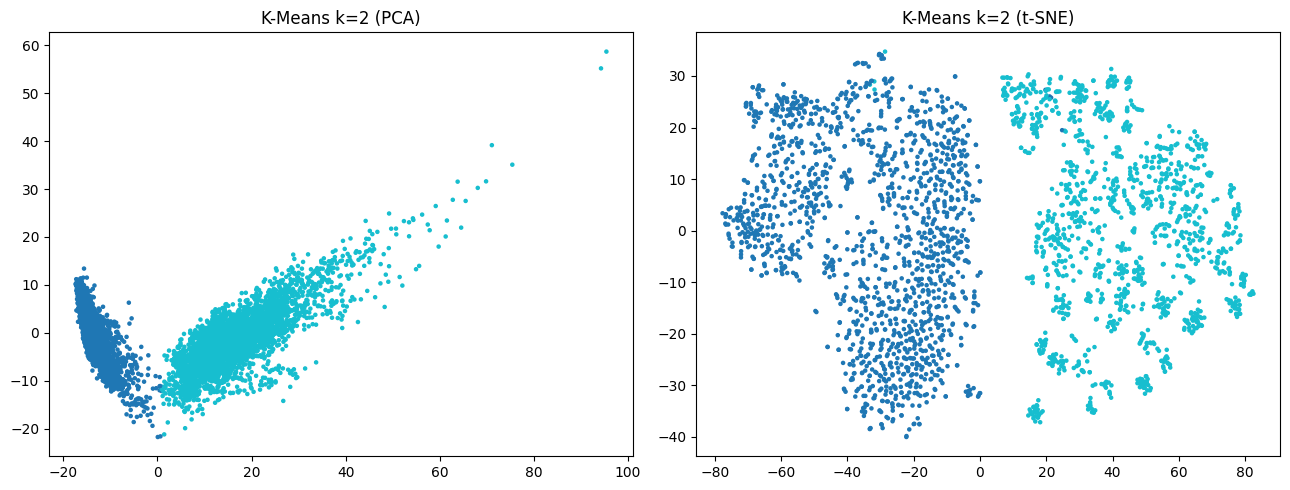
\includegraphics[width=0.9\linewidth]{kmeans_clusters_pca_tsne.png}
\caption{K-Means ($k=2$) Discovered Clusters Projected on PCA and t-SNE Spaces}
\end{figure}

\section{DBSCAN Density-Based Clustering}
DBSCAN discovers clusters of arbitrary shape by identifying core points with at least $minPts$ neighbors within distance $\epsilon$.

\subsection*{Figure: $k$-Distance Graph for Epsilon Estimation}
\begin{figure}[H]
\centering
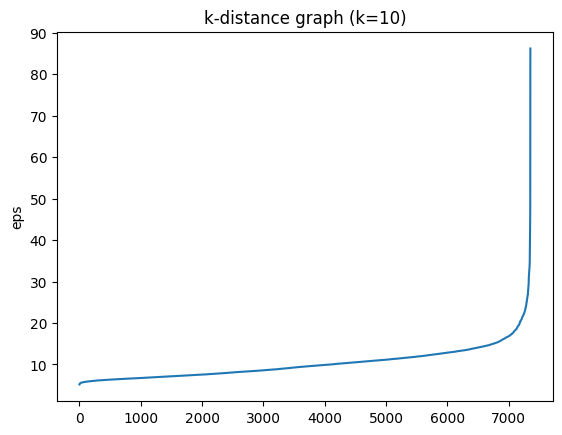
\includegraphics[width=0.65\linewidth]{dbscan_kdistance_graph.png}
\caption{$k$-Nearest Neighbor Distance Graph ($k=10$) for DBSCAN $\epsilon$ Threshold Selection}
\end{figure}

\textbf{Inference:}
Evaluating sorted 10-NN distances in the 50-dimensional PCA space shows an inflection point between $\epsilon = 11.0$ and $\epsilon = 13.0$. A systematic grid search was executed over candidate percentiles and $minPts \in \{5, 10, 20\}$.

\begin{table}[H]
\centering
\caption{DBSCAN Hyperparameter Grid Search on 50-Dimensional PCA Subspace}
\label{tab:dbscan_grid}
\begin{tabular}{|c|c|c|c|c|}
\hline
\textbf{Epsilon ($\epsilon$)} & \textbf{minPts} & \textbf{Clusters Formed} & \textbf{Noise Points ($l=-1$)} & \textbf{Silhouette Score}\\ \hline
11.35 & 5 & 18 & 1154 & 0.349\\ \hline
\textbf{11.35} & \textbf{10} & \textbf{9} & \textbf{1411} & \textbf{0.385}\\ \hline
11.35 & 20 & 3 & 1762 & 0.373\\ \hline
12.58 & 5 & 7 & 653 & 0.051\\ \hline
12.58 & 10 & 6 & 830 & 0.225\\ \hline
12.58 & 20 & 4 & 1140 & 0.306\\ \hline
14.45 & 5 & 2 & 298 & 0.381\\ \hline
14.45 & 10 & 2 & 385 & 0.339\\ \hline
14.45 & 20 & 2 & 498 & 0.339\\ \hline
\end{tabular}
\end{table}

\textbf{Inference:}
The parameter set $\epsilon = 11.35, minPts = 10$ achieved the highest non-trivial Silhouette score (\textbf{0.385}), isolating 9 dense local activity manifolds while classifying transitional movements (19.19\% of samples) as boundary noise.

\subsection*{Figure: DBSCAN Cluster Projection}
\begin{figure}[H]
\centering
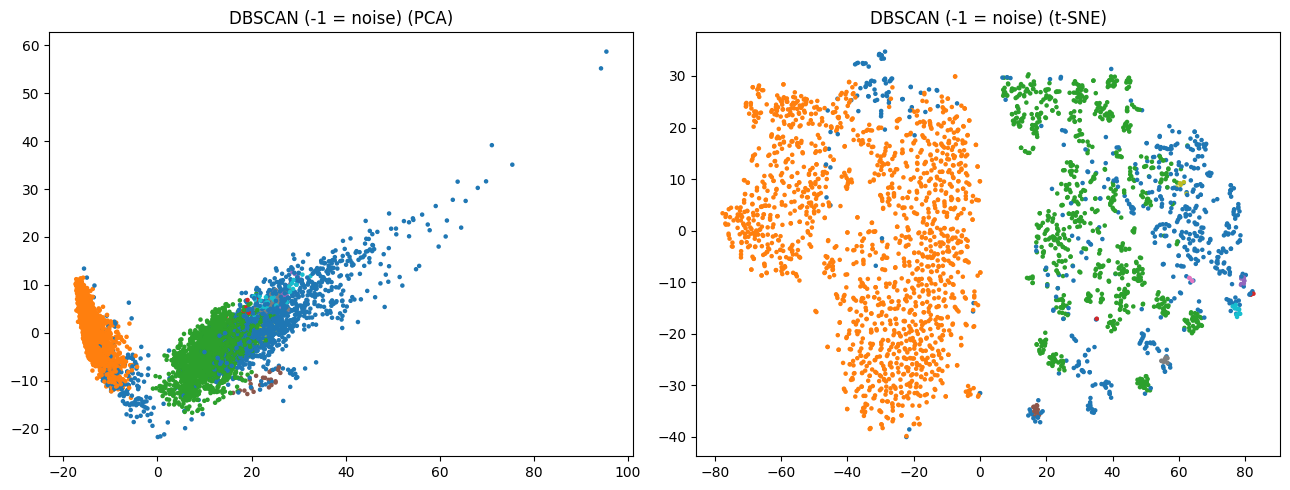
\includegraphics[width=0.9\linewidth]{dbscan_clusters_pca_tsne.png}
\caption{DBSCAN Density Clusters and Noise Identifications (PCA vs. t-SNE)}
\end{figure}

\section{Hierarchical Agglomerative Clustering (HAC)}
Hierarchical clustering builds a bottom-up tree based on pairwise proximity between sets of points:
\begin{table}[H]
\centering
\caption{Comparison of Linkage Criteria for Agglomerative Clustering ($K=6$)}
\label{tab:hac_linkages}
\begin{tabular}{|l|c|c|c|c|c|}
\hline
\textbf{Linkage Method} & \textbf{Silhouette} & \textbf{Davies-Bouldin} & \textbf{Calinski-Harabasz} & \textbf{ARI} & \textbf{NMI}\\ \hline
\textbf{HAC (Ward)} & \textbf{0.083} & \textbf{2.786} & \textbf{1730.84} & \textbf{0.279} & \textbf{0.454}\\ \hline
HAC (Complete) & 0.304 & 1.401 & 506.00 & 0.048 & 0.148\\ \hline
HAC (Average) & 0.516 & 0.655 & 32.59 & 0.000 & 0.003\\ \hline
HAC (Single) & 0.545 & 0.281 & 26.11 & 0.000 & 0.002\\ \hline
\end{tabular}
\end{table}

\textbf{Inference:}
Single and average linkage suffer from the \textit{chaining phenomenon}, merging nearly all samples into a single giant cluster and isolating single-point outliers (resulting in near-zero ARI and NMI). In contrast, \textbf{Ward's linkage} (which minimizes within-cluster variance) produces balanced clusters that closely match true activity distributions ($ARI = 0.279, NMI = 0.454$).

\subsection*{Figure: Hierarchical Clustering Dendrograms}
\begin{figure}[H]
\centering
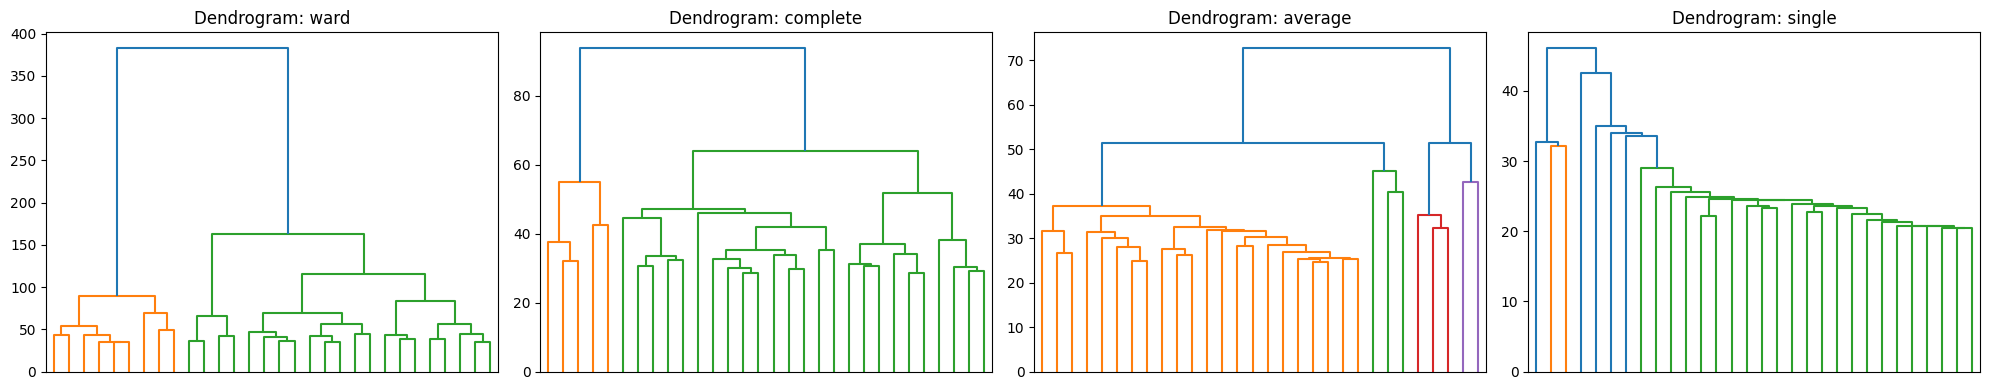
\includegraphics[width=0.95\linewidth]{hac_dendrograms.png}
\caption{Truncated Dendrograms (30 Root Branches) for Ward, Complete, Average, and Single Linkages}
\end{figure}

\subsection*{Figure: HAC Ward Clusters in PCA and t-SNE}
\begin{figure}[H]
\centering
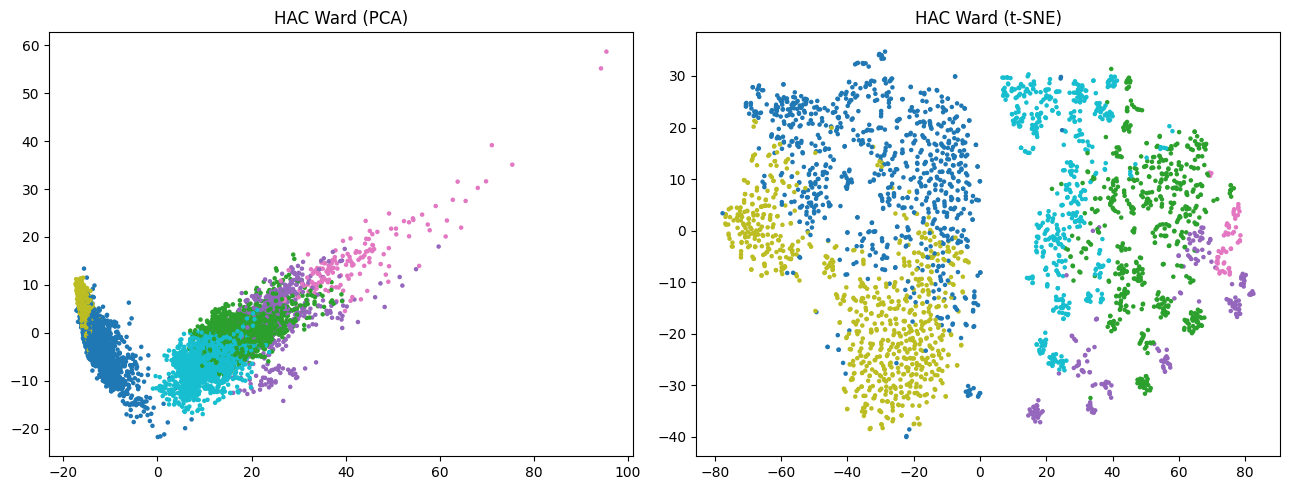
\includegraphics[width=0.9\linewidth]{hac_ward_clusters_pca_tsne.png}
\caption{HAC (Ward's Minimum Variance Linkage) 6-Cluster Projection on PCA and t-SNE}
\end{figure}

\section{Comprehensive Clustering Model Benchmark}
Table~\ref{tab:final_benchmark} compares the optimal configurations of all three clustering paradigms across intrinsic clustering quality metrics and extrinsic ground-truth alignment.

\begin{table}[H]
\centering
\caption{Comprehensive Clustering Benchmark on UCI HAR Dataset}
\label{tab:final_benchmark}
\begin{tabular}{|l|c|c|c|c|c|}
\hline
\textbf{Clustering Algorithm} & \textbf{Silhouette ($\uparrow$)} & \textbf{Davies-Bouldin ($\downarrow$)} & \textbf{Calinski-Harabasz ($\uparrow$)} & \textbf{ARI ($\uparrow$)} & \textbf{NMI ($\uparrow$)}\\ \hline
\textbf{K-Means ($k=2$)} & \textbf{0.397} & \textbf{1.069} & \textbf{5626.01} & \textbf{0.328} & \textbf{0.543}\\ \hline
\textbf{DBSCAN ($\epsilon=11.35, minPts=10$)} & 0.385 & 1.115 & 962.95 & 0.324 & 0.479\\ \hline
\textbf{HAC (Ward, $K=6$)} & 0.083 & 2.786 & 1730.84 & 0.279 & 0.454\\ \hline
\end{tabular}
\end{table}

\subsection*{Figure: Multi-Metric Benchmark Comparison}
\begin{figure}[H]
\centering
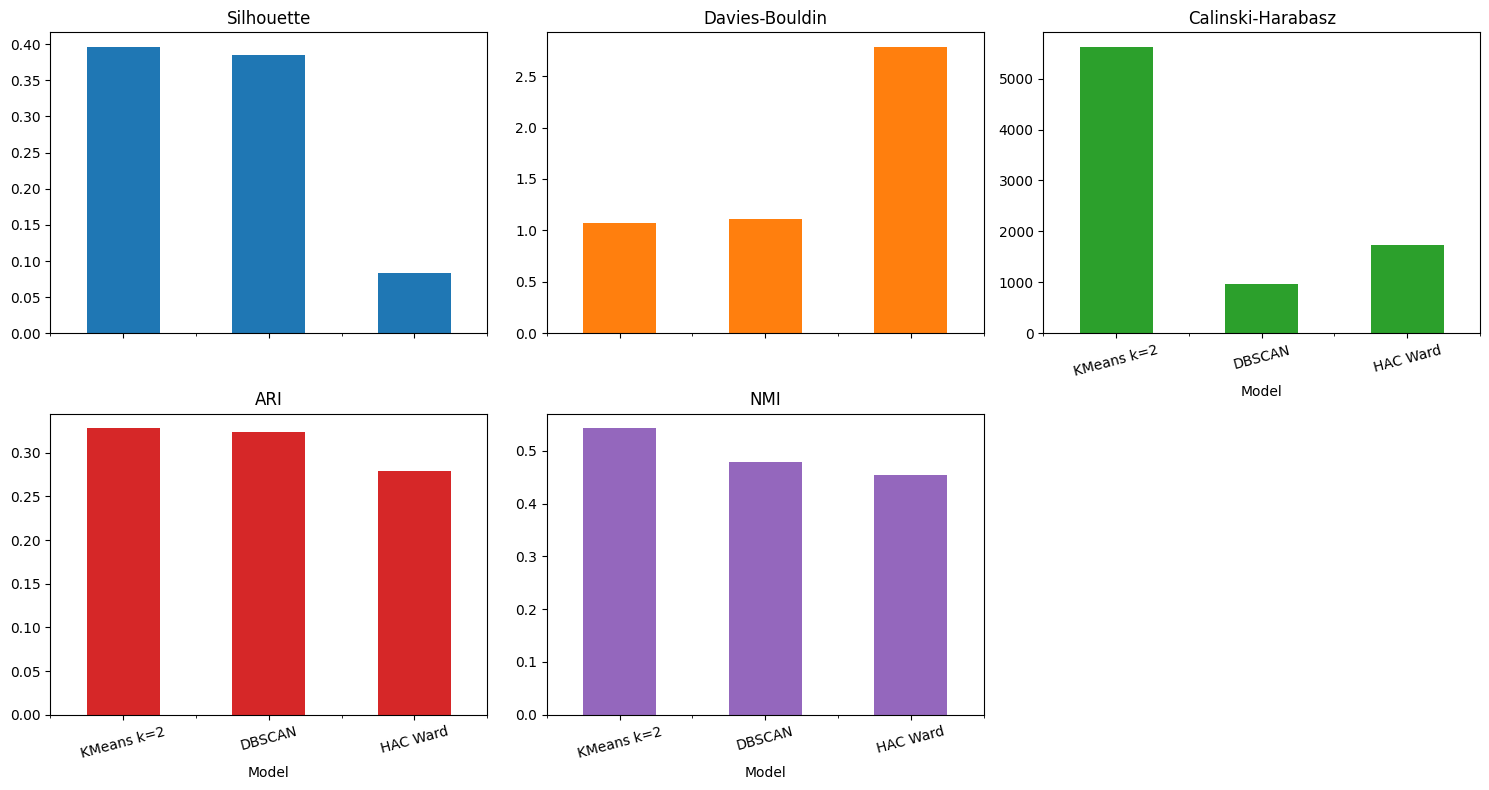
\includegraphics[width=0.95\linewidth]{clustering_metrics_comparison.png}
\caption{Bar Chart Comparison Across Silhouette, Davies-Bouldin, Calinski-Harabasz, ARI, and NMI}
\end{figure}

\section{Discussion and Analytical Observations}
\begin{enumerate}[leftmargin=*]
    \item \textbf{Cluster Separation vs. Sub-Activity Granularity:} K-Means with $k=2$ achieved the highest Silhouette score (0.397) and NMI (0.543) by capturing the fundamental physics separating dynamic acceleration from static orientation. Differentiating fine sub-activities (e.g., Sitting vs. Standing) requires non-Euclidean or supervised discriminative boundaries.
    \item \textbf{Density-Based Performance in High Dimensions:} In the original 561-dimensional space, pairwise distances become nearly equidistant due to metric concentration. Projecting onto a 50-dimensional PCA subspace enabled DBSCAN to effectively detect high-density cores while isolating 1,411 transitional noise records.
    \item \textbf{Linkage Criteria Sensitivity:} Ward's minimum variance linkage proved dramatically superior to single/average linkage, preventing chaining artifacts and producing compact, spherical activity partitions.
\end{enumerate}

\section{Experimental Setup}
\begin{longtable}{|p{6cm}|p{8cm}|}
\hline
Python Version & 3.11.x\\ \hline
Scikit-Learn Version & 1.6.1\\ \hline
SciPy Version & 1.11.x\\ \hline
IDE & Google Colab / Local Jupyter Notebook\\ \hline
Operating System & Windows 11\\ \hline
Hardware Platform & x86\_64 Multicore Processor\\ \hline
\end{longtable}

\section{Source Code and Implementation}
The complete Python code from \texttt{MLEXP8.ipynb} executing the clustering pipeline and metric evaluation is provided below:

\begin{lstlisting}
import numpy as np, pandas as pd, matplotlib.pyplot as plt, seaborn as sns
from sklearn.preprocessing import StandardScaler, LabelEncoder
from sklearn.decomposition import PCA
from sklearn.manifold import TSNE
from sklearn.neighbors import NearestNeighbors
from sklearn.cluster import KMeans, DBSCAN, AgglomerativeClustering
from sklearn.metrics import (
    silhouette_score, davies_bouldin_score,
    calinski_harabasz_score, adjusted_rand_score,
    normalized_mutual_info_score
)
from scipy.cluster.hierarchy import linkage, dendrogram

# 1. Load HAR Dataset
D = "/content/UCI HAR Dataset/"
X = pd.read_csv(D + "train/X_train.txt", sep=r"\s+", header=None)
y = pd.read_csv(D + "train/y_train.txt", header=None)[0]
acts = pd.read_csv(D + "activity_labels.txt", sep=r"\s+", header=None, index_col=0)[1]

X = X.fillna(X.median())
le = LabelEncoder()
y = le.fit_transform(y.map(acts))
Xs = StandardScaler().fit_transform(X)

# 2. Dimensionality Reductions
X2 = PCA(2).fit_transform(Xs)
X50 = PCA(50).fit_transform(Xs)
idx = np.random.RandomState(0).choice(len(Xs), 3000, replace=False)
T = TSNE(2, init="pca", random_state=0).fit_transform(Xs[idx])

# 3. K-Means Evaluation
ks = list(range(2, 9))
kms = [KMeans(k, n_init=10, random_state=0).fit(Xs) for k in ks]
wcss = [m.inertia_ for m in kms]
sil = [silhouette_score(Xs, m.labels_) for m in kms]
best_k = ks[int(np.argmax(sil))]
km = kms[ks.index(best_k)]

# 4. DBSCAN Tuning on 50D PCA Subspace
kd = np.sort(NearestNeighbors(n_neighbors=10).fit(X50).kneighbors(X50)[0][:, -1])
db = DBSCAN(eps=11.35, min_samples=10).fit_predict(X50)

# 5. Hierarchical Agglomerative Clustering
def evaluate_metrics(name, Z, l):
    m = l != -1
    ok = len(set(l[m])) > 1
    return {
        "Model": name,
        "Silhouette": silhouette_score(Z[m], l[m]) if ok else np.nan,
        "Davies-Bouldin": davies_bouldin_score(Z[m], l[m]) if ok else np.nan,
        "Calinski-Harabasz": calinski_harabasz_score(Z[m], l[m]) if ok else np.nan,
        "ARI": adjusted_rand_score(y, l),
        "NMI": normalized_mutual_info_score(y, l)
    }

hac = AgglomerativeClustering(n_clusters=6, linkage="ward").fit_predict(Xs)

# 6. Final Comparative Results
res = pd.DataFrame([
    evaluate_metrics(f"KMeans k={best_k}", Xs, km.labels_),
    evaluate_metrics("DBSCAN", X50, db),
    evaluate_metrics("HAC Ward", Xs, hac)
]).set_index("Model")
print(res.round(3))
\end{lstlisting}

\section{References}
\begin{enumerate}
    \item D. Arthur and S. Vassilvitskii, ``k-means++: The advantages of careful seeding,'' in \textit{Proc. ACM-SIAM SODA}, 2007, pp. 1027--1035.
    \item M. Ester, H.-P. Kriegel, J. Sander, and X. Xu, ``A density-based algorithm for discovering clusters in large spatial databases with noise,'' in \textit{Proc. KDD}, 1996, vol. 96, pp. 226--231.
    \item L. van der Maaten and G. Hinton, ``Visualizing data using t-SNE,'' \textit{Journal of Machine Learning Research}, vol. 9, pp. 2579--2605, 2008.
    \item D. Anguita et al., ``A public domain dataset for human activity recognition using smartphones,'' in \textit{ESANN}, 2013.
    \item F. Pedregosa et al., ``Scikit-learn: Machine learning in Python,'' \textit{Journal of Machine Learning Research}, vol. 12, pp. 2825--2830, 2011.
\end{enumerate}

\end{document}
